\documentclass[onecolumn,12pt]{IEEEtran}
\usepackage{etex}

\setlength{\marginparwidth}{20mm}
%\usepackage[disable]{todonotes}
%\usepackage{times}
\usepackage{helvet}
\usepackage{courier}
\usepackage{paralist}
\usepackage{latexsym}
\usepackage{url}
\usepackage[all]{xy}
%\usepackage{amsmath}
%\usepackage{amssymb}
%\usepackage{amsthm}
\usepackage{nccmath} % mfrac
\usepackage{comment}
%\usepackage{enumitem}
\usepackage{paralist}
% Adding back references to bib entries:
%\usepackage[colorlinks=true,linkcolor=blue,citecolor=purple,pagebackref=true]{hyperref}
%\usepackage[colorlinks=true,linkcolor=blue,citecolor=purple]{hyperref}
%\usepackage{hyperref}
\usepackage[dvipsnames]{xcolor}
\definecolor{lightgray}{gray}{0.9}
\usepackage{graphicx}
\usepackage{pifont}
%\usepackage{natbib}
%\usepackage{algorithm}
%\usepackage{algorithmic}
%\usepackage{pseudocode}
%\usepackage{algpseudocode}
\usepackage{savesym}
\savesymbol{AND}
\usepackage{xspace}
%\usepackage{pgf}
\usepackage{natbib}
\usepackage{algorithm}
\usepackage{algorithmic}
\usepackage{xspace}
\usepackage{tikz,pgfplots,placeins,comment}
\usepgfplotslibrary{external} 
\tikzexternalize
\pgfplotsset{compat=newest}
%\usepackage[capitalize]{cleveref}

%\pgfplotsset{filter discard warning=false}
%\usepgfplotslibrary{external} 
%\tikzexternalize[optimize=false] 
%\usepackage{style/ssltr}
%\usepackage{style/macros}
\usetikzlibrary{intersections}
\usetikzlibrary{arrows,calc,fit,patterns,plotmarks,shapes.geometric,shapes.misc,shapes.symbols,   shapes.arrows,   shapes.callouts,   shapes.multipart,   shapes.gates.logic.US,   shapes.gates.logic.IEC,   er,   automata,   backgrounds,   chains,   topaths,   trees,   petri,   mindmap,   matrix,   calendar,   folding, fadings,   through,   positioning,   scopes,   decorations.fractals,   decorations.shapes,   decorations.text,   decorations.pathmorphing,   decorations.pathreplacing,   decorations.footprints,   decorations.markings, shadows,circuits}
\usetikzlibrary{calc,trees,positioning,arrows,fit,shapes,calc}
\usetikzlibrary{calc,trees,positioning,arrows,chains,shapes.geometric,%
    shapes,shadows,matrix}
\tikzstyle{decision}=[diamond,draw]
\tikzstyle{line}=[draw]
\tikzstyle{elli}=[draw,ellipse]
\tikzstyle{arrow} = [thick]

\usepgfplotslibrary{external} 
\tikzexternalize
\pgfplotsset{compat=newest}

%\usepackage{subfig}
\newcommand{\mb}{\mbox{ }}
\newcommand{\one}{\mathbf{1}}
\newcommand{\zero}{\mathbf{0}}
\newcommand{\dr}{\delta}
\newcommand{\nn}{\nonumber}
\newcommand{\minp}{(\min,+)}
\newcommand{\maxp}{(\max,+)}
\newcommand{\V}{\mathcal{V}}
\newcommand{\R}{\mathbf{R}}
\newcommand{\Rm}{\mathbf{R}_{\min}}
\newcommand{\Ls}{\mathcal{L}}
\newcommand{\ra}{\rightarrow}
\newcommand{\om}{\otimes}
\newcommand{\op}{\oplus}
\newcommand{\nd}{n\times d}
\newcommand{\RA}{\Rightarrow}
\newcommand{\LA}{\Leftarrow}
\newcommand{\E}{\mathbf{E}}
\newcommand{\T}{\mathcal{T}}
\newcommand{\B}{\mathcal{B}}
\newcommand{\F}{\mathcal{F}}
\newcommand{\C}{\mathcal{C}}
\newcommand{\M}{\mathcal{M}}
\newcommand{\N}{\mathcal{N}}
\newcommand{\et}{||\Gamma J^*-\hg J^*||_\infty}
\newcommand{\etmn}{||\Gamma J^*-\hg J^*||_{\mn}}
\newcommand{\ini}{\lceil \frac{n}{k}\rceil}
\newcommand{\I}{\mathcal{I}}
\newcommand{\mut}{\tilde{\mu}}
\newcommand{\mn}{\infty,1/\psi}
\newcommand{\tj}{\tilde{J}_c}
\newcommand{\hj}{\hat{J}_c}
\newcommand{\jd}{J'_c}
\newcommand{\bj}{\bar{J}}
%\newcommand{\tv}{\tilde{V}}
\newcommand{\hv}{\hat{V}}

\newcommand{\tv}{V}
\newcommand{\tu}{\tilde{u}}
\newcommand{\hu}{\hat{u}}

\newcommand{\muh}{\hat{\mu}}
\newcommand{\mui}{{\mu}^i}

\newcommand{\br}{\bar{r}}
\newcommand{\hr}{\hat{r}_c}
\newcommand{\tr}{\tilde{r}_c}

\newcommand{\cf}{\mathcal{F}}
\newcommand{\X}{\mathcal{X}}



\newcommand{\norm}[1]{\|#1\|}
\newcommand{\inorm}[1]{\|#1\|_{\infty}}
\newcommand{\snorm}[1]{\left\|#1\right\|}
\newcommand{\sinorm}[1]{\left\|#1\right\|_{\infty}}




\newcommand{\tg}{\tilde{\Gamma}}
\newcommand{\har}{\hat{r}}


\newcommand{\conf}{\sqrt{\frac{2\ln t}{t_i}}}
%\newcommand{\tg}{\tilde{\Gamma}}
\newcommand{\hg}{\hat{\Gamma}}
\newcommand{\gd}{\Gamma'}
\newcommand{\vd}{V'}
%\newcommand{\qed}{\blacksquare}
\newcommand{\eps}{\varepsilon}
\renewcommand{\epsilon}{\varepsilon}


%\newenvironment{proof}{{\bf Proof:} }{}
%\newtheorem{theorem}{Theorem}
%\newtheorem{lemma}[theorem]{Lemma}
\newtheorem{assumption}{Assumption}
%\newtheorem{definition}[theorem]{Definition}
%\newtheorem{proposition}[theorem]{Proposition}
%\newtheorem{corollary}{Corollary}
\newtheorem{remark}{Remark}
%\newtheorem{example}{Example}
%\newtheorem{note}{Note}
%\newcommand{\alert}[1]{\textcolor{red}{#1}} 

\newcommand{\eqdef}{\stackrel{\Delta}{=}}

\def\v{\mathbf{v}}
\def\r{\mathbf{r}}
\def\p{\mathbf{p}}
\def\q{\mathbf{q}}
\def\R{\mathrm{R}}
\def\Re{\mathbb{R}}
\def\Z{\mathbb{Z}}
\def\P{\mathrm{P}}
\def\S{\mathcal{S}}
\def\A{\mathcal{A}}

\newcommand{\ith}[2][th]{$#2^{\text{#1}}$}

\newcounter{subequation}[equation]
\newcommand{\thesubequationonly}{\alph{subequation}}
\renewcommand{\thesubequation}{\text{\theequation(\thesubequationonly)}}
\newcommand{\subequationitem}{\refstepcounter{subequation}(\thesubequationonly)\thinspace}

\def\mathdisplay#1{%
  \ifmmode \@badmath
  \else
    $$\def\@currenvir{#1}%
    \let\dspbrk@context\z@
    \let\tag\tag@in@display \SK@equationtrue %\let\label\label@in@display
    \global\let\df@label\@empty \global\let\df@tag\@empty
    \global\tag@false
    \let\mathdisplay@push\mathdisplay@@push
    \let\mathdisplay@pop\mathdisplay@@pop
    \if@fleqn
      \edef\restore@hfuzz{\hfuzz\the\hfuzz\relax}%
      \hfuzz\maxdimen
      \setbox\z@\hbox to\displaywidth\bgroup
        \let\split@warning\relax \restore@hfuzz
        \everymath\@emptytoks \m@th $\displaystyle
    \fi
%   \fi
}

\newcommand{\algorithmicinput}{\textbf{Input:} }
\newcommand{\INPUT}{\item[\algorithmicinput]}
\newcommand{\algorithmicoutput}{\textbf{Output:} }
\newcommand{\OUTPUT}{\item[\algorithmicoutput]}
\newcounter{algostep}
\newcommand{\Step}[1][\STATE]{#1\textbf{\refstepcounter{algostep}\thealgostep}. }

\newenvironment{algoequation}{\refstepcounter{equation}$}{$\hfill (\theequation)}

\newenvironment{nonfloatalgorithm}[1]{\vspace{1ex}\hrule\vspace{0.5ex} \refstepcounter{algorithm}\textbf{Algorithm \thealgorithm}\hspace{1em} #1 \vspace{0.5ex}\hrule}{\hrule\vspace{1.5ex}\setcounter{algostep}{0}}

\newcounter{acalgorithm}

\newenvironment{nonfloatactorcriticalgorithm}[1]{\vspace{1ex}\hrule\vspace{0.5ex} \textbf{Actor-Critic Algorithm \refstepcounter{acalgorithm}\theacalgorithm}\hspace{1em} #1 \vspace{0.5ex}\hrule\addcontentsline{loa}{algorithm}{\protect\numberline{\theacalgorithm}{\ignorespaces #1}}}{\hrule\vspace{1.5ex}\setcounter{algostep}{0}}

\title{\large Research Statement\\Algorithms for Stochastic Control: Design, Analysis and Applications}
\author{Chandrashekar Lakshminarayanan}
\usepackage{caption}
\usepackage{cleveref}[capital]
\usepackage{tikz}
\begin{document}
%\Huge
%\begin{center}
%Panel of Experts
%\end{center}
\maketitle
%\input{abstract}

%Algorithms for stochastic control has been my area of research for the past eight years and I plan to continue working in the same area.  In \Cref{past}, I discuss my past research and in \Cref{future}, I present the future research directions. The rest of this sections presents some of the key design aspects, tools and techniques related to algorithms for stochastic control.

\section{Introduction}\label{intro}
\textbf{ Stochastic Control Setting:} Real world systems are (i) uncertain: that is, there is randomness (e.g., the time taken to service a customer in a queue, or the return-on-investment of a particular stock), (ii) complex: too many configurations (such as possible positions in a game of chess, or possible configurations of vehicular traffic in a big city), (iii) dynamic: the system configuration changes with time (number of customers in a queue, the price of a stock). However, the dynamics of such systems also depends on the decisions that we make from time to time (e.g., investment portfolio, moving a chess-piece, traffic signaling etc). 
An immediate question is that of \emph{optimal control} of such systems: can we come up with the right sequence of decisions?
\FloatBarrier
\begin{figure}[H]
\begin{minipage}[b]{0.5\textwidth}

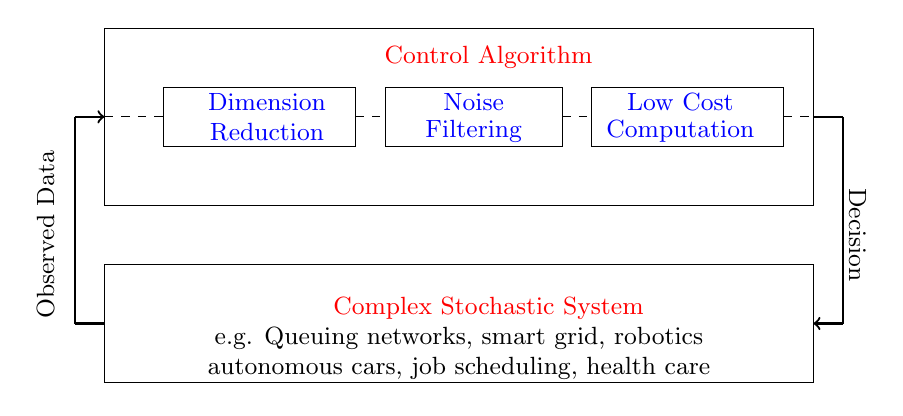
\begin{tikzpicture}[scale=0.75,font=\small,axis/.style={very thick, ->}]
%\draw [black](-2.25,-1) rectangle (2.25,2);
%\node[blue] at(0,1.75) {Modelling};
%\node[blue] at(-1.5,-1.5) {MDP};
%\node[blue] at(-1.5,-1.8) {\&};
%\node[blue] at(-1.5,-2.1) {SMPL};
%\draw[thick,->](-1.5,-1.4)--(-1.5,-0.75);






%\node[blue] at(8,-1.5) {ADP,RL,SPSA};
%\node[blue] at(8,-1.8) {\&};
%\node[blue] at(8,-2.1) {RL};

%\draw[thick,->](8,-1.4)--(8,0.1);
\node[red] at(4.5,4.5) {Control Algorithm};
\draw[black](-2,5) rectangle (10,2);


\draw [black](-1,3) rectangle (2.25,4);
\node[blue] at(.75,3.75) {Dimension};
\node[blue] at(.75,3.25) {Reduction};

\draw [black](5.75,3) rectangle (2.75,4);
\node[blue] at(4.25,3.75) {Noise};
\node[blue] at(4.25,3.25) {Filtering};

\draw [black](6.25,3) rectangle (9.5,4);
\node[blue] at(7.75,3.75) {Low Cost};
\node[blue] at(7.75,3.25) {Computation};

\node[red] at(4.5,0.25) {Complex Stochastic System};
\node[black] at(4,-0.25) {e.g. Queuing networks, smart grid, robotics};
\node[black] at(4,-0.75) {autonomous cars, job scheduling, health care};
\draw[black](-2,1) rectangle (10,-1);

\draw[thick,->](-2.5,3.5)--(-2,3.5);
\draw[thick,-](-2.5,3.5)--(-2.5,0);
\draw[thick,-](-2.5,0)--(-2,0);

\draw[dashed,-](-2,3.5)--(-1,3.5);
\draw[dashed,-](2.25,3.5)--(2.75,3.5);
\draw[dashed,-](5.75,3.5)--(6.25,3.5);
\draw[dashed,-](9.5,3.5)--(10,3.5);

\draw[thick,-](10,3.5)--(10.5,3.5);
\draw[thick,-](10.5,3.5)--(10.5,0);
\draw[thick,->](10.5,0)--(10,0);


\node[rotate=90] at(-3,1.5) {Observed Data};
\node[rotate=270] at(10.75,1.5) {Decision};

\end{tikzpicture}

\end{minipage}
\begin{minipage}[b]{0.5\textwidth}
\centering
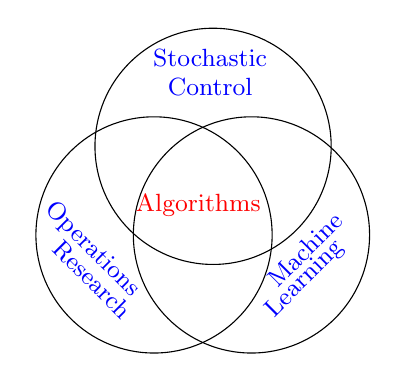
\begin{tikzpicture}[scale=0.75,font=\small,axis/.style={very thick, ->}]
\draw [] (0.9,0.5) circle (2);
\draw [] (-0.75,0.5) circle (2);
\draw [] (.25,2) circle (2);
%\draw [] (-0.5,0.5) circle (2);
%\draw [] (0.5,-0.5) circle (2);
%\draw [] (-0.5,-0.5) circle (2);

\node[red] at(0,1){Algorithms};
%\node[red] at(0,0.5) {Control};
\node[blue,rotate=45] at(1.8,.25){Machine};
\node[blue,rotate=45] at(1.8,-0.25){Learning};

\node[blue,rotate=-45] at(-1.8,.25){Operations};
\node[blue,rotate=-45] at(-1.8,-0.25){Research};

\node[blue] at(0.2,3.5){Stochastic};
\node[blue] at(0.2,3){Control};
\end{tikzpicture}

\end{minipage}


\label{plan}
\captionsetup{font=footnotesize}
\captionof{figure}{On the left is a schematic of a data-driven control algorithm; the observed data is mapped to a decision rule. The challenge is to design control algorithms that are data efficient, computationally cheap and scalable. The right diagram shows the overlap between three areas. Stochastic control has been used to address problems in operations research in the past. A recent trend has been to used machine learning techniques to build data-driven control algorithms.}
\end{figure}

\textbf{Objectives:}  As many applications are added by the day, and with the growing complexity, it is imperative to deploy algorithms to compute the decision rules (henceforth to be called as \emph{policies}), an otherwise impossible task for solely analytical methods or heuristics.  It is desirable for such control algorithms to satisfy the following (non-exhaustive) list of design objectives:
\begin{itemize}%[leftmargin=*]
\item Scalability: The number of configurations of the system grows exponentially in the number of dimensions.  It is desirable that the algorithms are computationally cheap, and are tractable. %For instance, consider a single traffic junction with $4$ lanes, and each lane with $3$ (low, medium, high) levels of traffic. The problem is completely specified by the $4$-dimensional quantity indicating the levels at the various lanes. However, the size of the state space is $3^4\approx 10^2$. The number of states in a big city with multiple junctions is exponentially large (say $\approx 10^{200}$ for $100$ junctions). Thus it is desirable for the computational costs to grow only as a function of the state variables and not the size of the state space.
 \item Data-Driven: In most scenarios, the underlying model parameters are not known and it becomes important for the algorithms to be solely data-driven. A closely related aspect is that of data efficiency, wherein the algorithms are expected to use all the available information in the given data samples.
\item Performance Guarantee: The algorithms need to be stable, i.e., should produce convergent policies. Further, it is desirable that the computed policy is near-optimal.
\end{itemize}

\textbf{Design tools and analysis techniques:} The schematic (Fig.~\ref{plan}) shows the overall template of a control algorithm that is likely to meet these design objectives. %Markov decision processes (MDPs) is a useful mathematical framework to formulate many stochastic control problems, and forms the basis for design and analysis of a wide family of control algorithms. 
While specific details of the algorithms could vary, all of them can be said to combine three keys components (not in any specific order) namely data assimilation, dimension reduction and low-cost computation. Markov decision processes (MDPs) is a useful tool to formulate stochastic control problems, and the Markovian nature gives rise to the idea of dynamic programming (DP) which forms the back bone of the computational procedure in most of such control algorithms. Ideas related to dimensionality reduction and data assimilation come from theory of approximate dynamic programming (ADP) and stochastic approximation (SA) respectively. Recent times have also seen the growth of a class of stochastic control algorithms called reinforcement learning (RL) algorithms which combine ideas of ADP and SA, and machine learning to learn policies in a data-driven manner. RL algorithms have been extremely successful in a variety of applications such as queuing networks, autonomous game play and robotics.
%The algorithms are in general sample trajectory versions of approximate dynamic programming that combine ideas of dimensionality reduction and dynamic programming, are model based and computationally cheap. Reinforcement learning algorithms are data-driven algorithms and in most cases are sample trajectory versions of ADP algorithms. RL algorithms are data-driven, and computationally cheap, and have been found to be successful in a variety of applications. Theoretical convergence of RL algorithms follow from stochastic approximation theory. 


\section{Past Work}\label{past}
In \cref{intro}, we saw some key design objectives and techniques for design of control algorithms. Naturally, the following questions are of interest: are computationally cheap, data-driven alogorithms stable? do they give useful policies? how fast do they estimate? where can we apply these algorithms? I was fortunate to contribute towards the answering some of these questions during the past years via design of new algorithms and novel analytical techniques as well as by developing control algorithms for practical applications.

\textbf{Scalabe ADP in $\minp$ basis:} 
%A widely used dimensionality reduction technique is linear function approximation, wherein, the value function is approximated by the linear combination of set of chosen basis functions. By choosing fewer basis functions (in comparison to the size of the state space), the ADP algorithm is dimension free.
One of the important issues with such ADP is that even the most fundamental methods such as approximate value iteration/policy iteration (AVI/API) don't have convergence guarantees, i.e., the computed sequence of policies can diverge. We \cite{cdc} showed that if the basis is chosen to be $\minp$ linear (also known as tropical-linearity), then the ADP methods will be convergent and performance loss of the computed policy can be bound analytically.

\textbf{Scalability via constraint reduction:} The approximate linear program (ALP) is an ADP method that has performance guarantees \cite{alp} for the computed policy and is guaranteed to converge (unlike other AVI/API). A limitation of the ALP is the intractably large number of constraints.  We \cite{alp-aaai,alp-ieee} provided theoretical guarantees for constraint reduction in ALP. Our arguments are based on the geometry of linear programs as opposed to previous works \cite{cs} based on counting (VC-dimension) based arguments. We showed that the performance can be guaranteed by choosing the constraints corresponding to a \emph{conic-cover} of the given basis functions.

\textbf{Stability:} We derived \cite{automatica} conditions that imply stability and boundedness of multi-timescale stochastic approximation (SA) algorithms. Our work significantly extended the prior work on the stability of single timescale SA algorithms \cite{borkar-meyn}, and provided a blanket result that covers widely used class of RL algorithms called actor-critic methods. 

\textbf{Finite-Time Performance:} Temporal difference (TD) class of learning algorithms have been widely used to learn value functions of a given policy. Such value function learning is a sub-loop in many important RL algorithms (such as actor-critic methods). Many of the important TD algorithms are also linear stochastic (LSA) approximation methods. The choice of the stepsize or learning rate is critical for the performance of LSA algorithms. We studied LSA with constant stepsize and iterative averaging \cite{aistats}, and showed they achieve a problem instance dependent optimal rate of convergence for the mean-squared estimation error. Our work eliminates stepsize tuning in a host of TD algorithms.

\textbf{Optimal Pricing:} Crowd-sourcing, in recent times, has been used to perform \emph{human intelligence tasks} (which are hard for computers) such as image annotation, transcription. The tasks are posted onto online platforms such as Amazon Mechanical Turk or Crowdflower, and workers can pick a task of their choice. The price offered is a critical factor that determines the time taken to complete a task.
 We collected real world data from Crowdflower and showed \cite{hcomp} that the learnt optimal pricing policy achieves better completion times.
 
 \textbf{High Dimension parameter tuning:} Apache Hadoop is a distributed storage and computing framework meant to handle big data. A key to faster computation is the parameter setting which dictates the allocation of resources within Hadoop. We proposed \cite{hadoop} a noisy gradient algorithm to tune the parameters in Hadoop framework; our approach achieved $25\%$ to $60\%$ improvement in performance over the default parameter setting.

%\textbf{Crowd-sourcing:} is a new paradigm wherein tasks that are difficult for computers but easy for humans are solved in a decentralized manner. Here, such tasks are posted on to crowd-sourcing platforms (such as Amazon Mechanical Turk, Crowdflower), to be picked by crowd-workers, who can finish such tasks in their free time. The price offered to the workers for completing is a critical factor that determines the time taken to complete the tasks.  In our work \cite{hcomp}, we considered the problem of optimal pricing of crowd-sourced tasks, with an aim to achieve timely completion. We collected real-time data from CrowdFlower, learnt the underlying MDP, solved for the optimal pricing policy and deployed the pricing policy in real-time, which achieved significant improvement over uncontrolled policies.

%\textbf{Hadoop:} The performance critically depends on tuning parameters.

\section{Future Work}\label{future}
 I strongly believe that new practical application problems give rise to new design objectives and algorithmic ideas.  Thus, I strive to strike a healthy balance between theoretical questions as well as practical problems in stochastic control. I am likely to pursue some of the following directions:
 
 \textbf{Constrained and Risk-Sensitive Control:} Several applications need policies to satisfy one or more constraints. For example, in energy harvesting sensor networks, each sensor is constrained by the amount of energy it can expend at any given time, or an autonomous driving system has speed limitations, or a stock investment policy cannot fluctuate the portfolios in a non-smooth manner. Another aspect is that of risk-sensitivity, i.e., the policies are not supposed to visit certain \emph{dangerous} states. For example, while controlling a helicopter, there could be states that lead to instability and eventually cause the overall system to crash. Thus, developing data-driven control algorithms for risk-sensitive and constrained control problems is an interesting research direction with a variety of applications.

 
 \textbf{Decentralized multi-agent control:} is an architecture wherein several controllers make decisions based on local information. Decentralization is done either to reduce computational costs or happens naturally due to geographical constraints, and these systems may or may not be networked via a communication protocol. The presence of multiple controllers induces a \emph{stochastic game}, and naturally solution concepts such as Shapely value or Nash equilibrium come into the picture. Designing data-driven multi-agent algorithms that converge to such equilibria is an interesting direction. Another related question is that of data-driven mechanism design which deals with allocating incentives to such selfish decentralized agents.

% \textbf{Exploration vs Exploitation:} An important stochastic control problem is that of efficient data assimilation, i.e., based on prior data we need a policy that learns about the environment in an optimal way. An example application is health care, wherein, it is important to gather maximum patient information while making minimal possible tests. Also, in many applications the feedback might be complex, i.e., we can obtain the rewards only for a group of actions (by several decentralized control units), or the feedback is delayed. Typically, these problems are posed as multi-armed bandit problems, while the independent arms case and the linear MAB problems have been well understood in literature, newer applications typically require significant modification of the basic MAB algorithms. In particular, multi-agent systems such as sensor networks, or robots, decentralized MAB algorithms are required for effective co-ordination via optimal communication.
  
 
 \textbf{Classical vs Learning based Control:} Classical control as well as learning based algorithms have the same objective, i.e., to produce useful decision rules. However, the approaches in both the areas are quite different. Classical control is mostly model-based and learning based algorithms do not worry about the model, but instead are geared towards design of solely data-driven controllers. Specifically, several learning control algorithms have deep neural networks (DNNs) as their integral part, and the following questions about DNNs are still open: when are DNNs trainable? why do DNNs generalize? when do DNNs produce reliable policies? An interesting research direction is to use tools from control theory to answer some of the questions. For instance, optimization algorithms used in training such as Nestrov's accelerated gradient have been interpreted as dynamical systems \cite{ben}, and tools from robust control theory have been used for principled design of these algorithms. As we move forward to newer applications, combining tools and techniques from both classical and learning based control to design and analyze hybrid controllers is of interest.
 
 \textbf{Vision and Control:} A common thread connecting some of the recent success of learning based control such as Atari, AlphaGo and autonomous driving is that the input is a vision signal.  A general view is that the vision signals are rich in representing the underlying environment and by learning the inherent symmetries in the vision input can help in efficient control. This leads to an interesting question \cite{vision} in the other direction: can control policies also dictate attention towards particular parts in the field of view to gain useful information? To answer these questions, it is important to pose combined vision and control problems to design newer algorithms.

 \textbf{Human-in-the-loop:} Learning based control algorithms are increasingly applied in domains such as \emph{mobile} healthcare \cite{mhealth}, automatic curriculum design (known as \emph{e-learning}) and crowd-sourcing \cite{crowd}. A common theme here is that the systems that are being controlled are humans. At the opposite end are techniques such as imitation learning \cite{il} where human beings can demonstrate/recommend optimal policies and the controller is supposed to learn from human behavior. In both these scenarios, the dynamics and behavior of the human beings plays a critical role. Investigating the effects of humans in the loop either as a controller or as the controlled system is an interesting research direction.
 
\section{Conclusion}
This document outlines some of my past and future research directions in the area of algorithms for stochastic control. These plans and directions are at various levels of concreteness; some of them require significant extension of existing theory, others require newer mathematical formulations. Most of these problems have well founded application areas as well. I also believe that these research directions are inherently flexible to cater the interests of most students. The list of directions are not exhaustive and I will constantly strive to add newer directions with the progress of time.
\bibliographystyle{plain}
\bibliography{refnew}

\end{document}
